\batchmode
\documentclass[twoside]{book}

% Packages required by doxygen
\usepackage{fixltx2e}
\usepackage{calc}
\usepackage{doxygen}
\usepackage[export]{adjustbox} % also loads graphicx
\usepackage{graphicx}
\usepackage[utf8]{inputenc}
\usepackage{makeidx}
\usepackage{multicol}
\usepackage{multirow}
\PassOptionsToPackage{warn}{textcomp}
\usepackage{textcomp}
\usepackage[nointegrals]{wasysym}
\usepackage[table]{xcolor}

% Font selection
\usepackage[T1]{fontenc}
\usepackage[scaled=.90]{helvet}
\usepackage{courier}
\usepackage{amssymb}
\usepackage{sectsty}
\renewcommand{\familydefault}{\sfdefault}
\allsectionsfont{%
  \fontseries{bc}\selectfont%
  \color{darkgray}%
}
\renewcommand{\DoxyLabelFont}{%
  \fontseries{bc}\selectfont%
  \color{darkgray}%
}
\newcommand{\+}{\discretionary{\mbox{\scriptsize$\hookleftarrow$}}{}{}}

% Page & text layout
\usepackage{geometry}
\geometry{%
  a4paper,%
  top=2.5cm,%
  bottom=2.5cm,%
  left=2.5cm,%
  right=2.5cm%
}
\tolerance=750
\hfuzz=15pt
\hbadness=750
\setlength{\emergencystretch}{15pt}
\setlength{\parindent}{0cm}
\setlength{\parskip}{3ex plus 2ex minus 2ex}
\makeatletter
\renewcommand{\paragraph}{%
  \@startsection{paragraph}{4}{0ex}{-1.0ex}{1.0ex}{%
    \normalfont\normalsize\bfseries\SS@parafont%
  }%
}
\renewcommand{\subparagraph}{%
  \@startsection{subparagraph}{5}{0ex}{-1.0ex}{1.0ex}{%
    \normalfont\normalsize\bfseries\SS@subparafont%
  }%
}
\makeatother

% Headers & footers
\usepackage{fancyhdr}
\pagestyle{fancyplain}
\fancyhead[LE]{\fancyplain{}{\bfseries\thepage}}
\fancyhead[CE]{\fancyplain{}{}}
\fancyhead[RE]{\fancyplain{}{\bfseries\leftmark}}
\fancyhead[LO]{\fancyplain{}{\bfseries\rightmark}}
\fancyhead[CO]{\fancyplain{}{}}
\fancyhead[RO]{\fancyplain{}{\bfseries\thepage}}
\fancyfoot[LE]{\fancyplain{}{}}
\fancyfoot[CE]{\fancyplain{}{}}
\fancyfoot[RE]{\fancyplain{}{\bfseries\scriptsize Generated by Doxygen }}
\fancyfoot[LO]{\fancyplain{}{\bfseries\scriptsize Generated by Doxygen }}
\fancyfoot[CO]{\fancyplain{}{}}
\fancyfoot[RO]{\fancyplain{}{}}
\renewcommand{\footrulewidth}{0.4pt}
\renewcommand{\chaptermark}[1]{%
  \markboth{#1}{}%
}
\renewcommand{\sectionmark}[1]{%
  \markright{\thesection\ #1}%
}

% Indices & bibliography
\usepackage{natbib}
\usepackage[titles]{tocloft}
\setcounter{tocdepth}{3}
\setcounter{secnumdepth}{5}
\makeindex

% Hyperlinks (required, but should be loaded last)
\usepackage{ifpdf}
\ifpdf
  \usepackage[pdftex,pagebackref=true]{hyperref}
\else
  \usepackage[ps2pdf,pagebackref=true]{hyperref}
\fi
\hypersetup{%
  colorlinks=true,%
  linkcolor=blue,%
  citecolor=blue,%
  unicode%
}

% Custom commands
\newcommand{\clearemptydoublepage}{%
  \newpage{\pagestyle{empty}\cleardoublepage}%
}

\usepackage{caption}
\captionsetup{labelsep=space,justification=centering,font={bf},singlelinecheck=off,skip=4pt,position=top}

%===== C O N T E N T S =====

\begin{document}

% Titlepage & ToC
\hypersetup{pageanchor=false,
             bookmarksnumbered=true
            }
\pagenumbering{alph}
\pagenumbering{arabic}
\hypersetup{pageanchor=true}

%--- Begin generated contents ---
\chapter{Example problem\+: Adaptive simulation of finite-\/\+Reynolds number entry flow into a 3D tube}
\label{index}\hypertarget{index}{}\hypertarget{index_q}{}\section{A few quick questions...}\label{index_q}
Since {\ttfamily oomph-\/lib} is developed as open-\/source software, any evidence that the code is being downloaded and used is very helpful for us as it helps to justify our continued work on this project.

We would therefore be extremely grateful if you could provide the information requested in the form below. Pressing the \char`\"{}submit\char`\"{} button will get you to the actual download page.

{\bfseries Note\+:} 
\begin{DoxyItemize}
\item All information will be treated as confidential. 
\item If you provide your email address and check the appropriate box we will add you to our mailing list to inform you of upgrades and bug fixes to the code. Rest assured that the mailing list is {\bfseries very low volume} -- we have better things to do than to bombard you with email. 
\item If you still feel reluctant to provide any of the information requested, feel free to enter some dummy input. The form will check that {\bfseries some} information has been entered but entering your name as \char`\"{}\+Joe Cool\char`\"{} is perfectly acceptable -- this is to discourage people from not providing the information simply because they are too lazy to type... 
\end{DoxyItemize}



 







 

 \hypertarget{index_pdf}{}\section{P\+D\+F file}\label{index_pdf}
A \href{../latex/refman.pdf}{\tt pdf version} of this document is available. \end{document}

\chapter{Namespace Index}
\section{Namespace List}
Here is a list of all namespaces with brief descriptions\+:\begin{DoxyCompactList}
\item\contentsline{section}{\hyperlink{namespaceGlobal__Physical__Variables}{Global\+\_\+\+Physical\+\_\+\+Variables} \\*Global variables that represent physical properties }{\pageref{namespaceGlobal__Physical__Variables}}{}
\item\contentsline{section}{\hyperlink{namespaceoomph}{oomph} }{\pageref{namespaceoomph}}{}
\item\contentsline{section}{\hyperlink{namespacePhysical__Variables}{Physical\+\_\+\+Variables} \\*Namespace for the solution of 2D linear shell equation }{\pageref{namespacePhysical__Variables}}{}
\end{DoxyCompactList}

\chapter{Hierarchical Index}
\section{Class Hierarchy}
This inheritance list is sorted roughly, but not completely, alphabetically\+:\begin{DoxyCompactList}
\item Problem\begin{DoxyCompactList}
\item \contentsline{section}{Unstructured\+Solid\+Problem$<$ E\+L\+E\+M\+E\+NT $>$}{\pageref{classUnstructuredSolidProblem}}{}
\end{DoxyCompactList}
\end{DoxyCompactList}

\chapter{Class Index}
\section{Class List}
Here are the classes, structs, unions and interfaces with brief descriptions\+:\begin{DoxyCompactList}
\item\contentsline{section}{\hyperlink{classPMLProblem}{P\+M\+L\+Problem$<$ E\+L\+E\+M\+E\+N\+T $>$} }{\pageref{classPMLProblem}}{}
\item\contentsline{section}{\hyperlink{classGlobalParameters_1_1TestPMLMapping}{Global\+Parameters\+::\+Test\+P\+M\+L\+Mapping} }{\pageref{classGlobalParameters_1_1TestPMLMapping}}{}
\end{DoxyCompactList}

\chapter{File Index}
\section{File List}
Here is a list of all files with brief descriptions\+:\begin{DoxyCompactList}
\item\contentsline{section}{\hyperlink{jeffery__orbit_8cc}{jeffery\+\_\+orbit.\+cc} }{\pageref{jeffery__orbit_8cc}}{}
\item\contentsline{section}{\hyperlink{jeffery__orbit_8txt__doxygenified_8h}{jeffery\+\_\+orbit.\+txt\+\_\+doxygenified.\+h} }{\pageref{jeffery__orbit_8txt__doxygenified_8h}}{}
\item\contentsline{section}{\hyperlink{my__taylor__hood__elements_8h}{my\+\_\+taylor\+\_\+hood\+\_\+elements.\+h} }{\pageref{my__taylor__hood__elements_8h}}{}
\end{DoxyCompactList}

\chapter{Namespace Documentation}
\hypertarget{namespaceGlobal__Physical__Variables}{}\section{Global\+\_\+\+Physical\+\_\+\+Variables Namespace Reference}
\label{namespaceGlobal__Physical__Variables}\index{Global\+\_\+\+Physical\+\_\+\+Variables@{Global\+\_\+\+Physical\+\_\+\+Variables}}


Namespace for physical parameters.  


\subsection*{Functions}
\begin{DoxyCompactItemize}
\item 
Vector$<$ double $>$ \hyperlink{namespaceGlobal__Physical__Variables_afae321364975eb56688ad13abc8ed6b7}{Gravity} (2)
\begin{DoxyCompactList}\small\item\em Gravity vector. \end{DoxyCompactList}\item 
void \hyperlink{namespaceGlobal__Physical__Variables_a87da705b8a46bed337cf5dbdd788b87b}{body\+\_\+force} (const double \&time, const Vector$<$ double $>$ \&x, Vector$<$ double $>$ \&result)
\begin{DoxyCompactList}\small\item\em Functional body force. \end{DoxyCompactList}\item 
void \hyperlink{namespaceGlobal__Physical__Variables_a9780d615ae07c4e00a436ab2973b54e6}{zero\+\_\+body\+\_\+force} (const double \&time, const Vector$<$ double $>$ \&x, Vector$<$ double $>$ \&result)
\begin{DoxyCompactList}\small\item\em Zero functional body force. \end{DoxyCompactList}\end{DoxyCompactItemize}
\subsection*{Variables}
\begin{DoxyCompactItemize}
\item 
double \hyperlink{namespaceGlobal__Physical__Variables_ab814e627d2eb5bc50318879d19ab16b9}{Re} =100
\begin{DoxyCompactList}\small\item\em Reynolds number. \end{DoxyCompactList}\item 
double \hyperlink{namespaceGlobal__Physical__Variables_ab1a845a672b4d74b304639a976dc65c6}{Re\+\_\+inv\+Fr} =100
\begin{DoxyCompactList}\small\item\em Reynolds/\+Froude number. \end{DoxyCompactList}\end{DoxyCompactItemize}


\subsection{Detailed Description}
Namespace for physical parameters. 

\subsection{Function Documentation}
\mbox{\Hypertarget{namespaceGlobal__Physical__Variables_a87da705b8a46bed337cf5dbdd788b87b}\label{namespaceGlobal__Physical__Variables_a87da705b8a46bed337cf5dbdd788b87b}} 
\index{Global\+\_\+\+Physical\+\_\+\+Variables@{Global\+\_\+\+Physical\+\_\+\+Variables}!body\+\_\+force@{body\+\_\+force}}
\index{body\+\_\+force@{body\+\_\+force}!Global\+\_\+\+Physical\+\_\+\+Variables@{Global\+\_\+\+Physical\+\_\+\+Variables}}
\subsubsection{\texorpdfstring{body\+\_\+force()}{body\_force()}}
{\footnotesize\ttfamily void Global\+\_\+\+Physical\+\_\+\+Variables\+::body\+\_\+force (\begin{DoxyParamCaption}\item[{const double \&}]{time,  }\item[{const Vector$<$ double $>$ \&}]{x,  }\item[{Vector$<$ double $>$ \&}]{result }\end{DoxyParamCaption})}



Functional body force. 



Definition at line 62 of file circular\+\_\+driven\+\_\+cavity.\+cc.



References Re\+\_\+inv\+Fr.



Referenced by main().

\mbox{\Hypertarget{namespaceGlobal__Physical__Variables_afae321364975eb56688ad13abc8ed6b7}\label{namespaceGlobal__Physical__Variables_afae321364975eb56688ad13abc8ed6b7}} 
\index{Global\+\_\+\+Physical\+\_\+\+Variables@{Global\+\_\+\+Physical\+\_\+\+Variables}!Gravity@{Gravity}}
\index{Gravity@{Gravity}!Global\+\_\+\+Physical\+\_\+\+Variables@{Global\+\_\+\+Physical\+\_\+\+Variables}}
\subsubsection{\texorpdfstring{Gravity()}{Gravity()}}
{\footnotesize\ttfamily Vector$<$double$>$ Global\+\_\+\+Physical\+\_\+\+Variables\+::\+Gravity (\begin{DoxyParamCaption}\item[{2}]{ }\end{DoxyParamCaption})}



Gravity vector. 



Referenced by main(), and Quarter\+Circle\+Driven\+Cavity\+Problem$<$ E\+L\+E\+M\+E\+N\+T $>$\+::\+Quarter\+Circle\+Driven\+Cavity\+Problem().

\mbox{\Hypertarget{namespaceGlobal__Physical__Variables_a9780d615ae07c4e00a436ab2973b54e6}\label{namespaceGlobal__Physical__Variables_a9780d615ae07c4e00a436ab2973b54e6}} 
\index{Global\+\_\+\+Physical\+\_\+\+Variables@{Global\+\_\+\+Physical\+\_\+\+Variables}!zero\+\_\+body\+\_\+force@{zero\+\_\+body\+\_\+force}}
\index{zero\+\_\+body\+\_\+force@{zero\+\_\+body\+\_\+force}!Global\+\_\+\+Physical\+\_\+\+Variables@{Global\+\_\+\+Physical\+\_\+\+Variables}}
\subsubsection{\texorpdfstring{zero\+\_\+body\+\_\+force()}{zero\_body\_force()}}
{\footnotesize\ttfamily void Global\+\_\+\+Physical\+\_\+\+Variables\+::zero\+\_\+body\+\_\+force (\begin{DoxyParamCaption}\item[{const double \&}]{time,  }\item[{const Vector$<$ double $>$ \&}]{x,  }\item[{Vector$<$ double $>$ \&}]{result }\end{DoxyParamCaption})}



Zero functional body force. 



Definition at line 70 of file circular\+\_\+driven\+\_\+cavity.\+cc.



Referenced by main().



\subsection{Variable Documentation}
\mbox{\Hypertarget{namespaceGlobal__Physical__Variables_ab814e627d2eb5bc50318879d19ab16b9}\label{namespaceGlobal__Physical__Variables_ab814e627d2eb5bc50318879d19ab16b9}} 
\index{Global\+\_\+\+Physical\+\_\+\+Variables@{Global\+\_\+\+Physical\+\_\+\+Variables}!Re@{Re}}
\index{Re@{Re}!Global\+\_\+\+Physical\+\_\+\+Variables@{Global\+\_\+\+Physical\+\_\+\+Variables}}
\subsubsection{\texorpdfstring{Re}{Re}}
{\footnotesize\ttfamily double Global\+\_\+\+Physical\+\_\+\+Variables\+::\+Re =100}



Reynolds number. 



Definition at line 53 of file circular\+\_\+driven\+\_\+cavity.\+cc.



Referenced by Quarter\+Circle\+Driven\+Cavity\+Problem$<$ E\+L\+E\+M\+E\+N\+T $>$\+::\+Quarter\+Circle\+Driven\+Cavity\+Problem().

\mbox{\Hypertarget{namespaceGlobal__Physical__Variables_ab1a845a672b4d74b304639a976dc65c6}\label{namespaceGlobal__Physical__Variables_ab1a845a672b4d74b304639a976dc65c6}} 
\index{Global\+\_\+\+Physical\+\_\+\+Variables@{Global\+\_\+\+Physical\+\_\+\+Variables}!Re\+\_\+inv\+Fr@{Re\+\_\+inv\+Fr}}
\index{Re\+\_\+inv\+Fr@{Re\+\_\+inv\+Fr}!Global\+\_\+\+Physical\+\_\+\+Variables@{Global\+\_\+\+Physical\+\_\+\+Variables}}
\subsubsection{\texorpdfstring{Re\+\_\+inv\+Fr}{Re\_invFr}}
{\footnotesize\ttfamily double Global\+\_\+\+Physical\+\_\+\+Variables\+::\+Re\+\_\+inv\+Fr =100}



Reynolds/\+Froude number. 



Definition at line 56 of file circular\+\_\+driven\+\_\+cavity.\+cc.



Referenced by body\+\_\+force(), and Quarter\+Circle\+Driven\+Cavity\+Problem$<$ E\+L\+E\+M\+E\+N\+T $>$\+::\+Quarter\+Circle\+Driven\+Cavity\+Problem().


\chapter{Class Documentation}
\hypertarget{classEntryFlowProblem}{}\section{Entry\+Flow\+Problem$<$ E\+L\+E\+M\+E\+NT $>$ Class Template Reference}
\label{classEntryFlowProblem}\index{Entry\+Flow\+Problem$<$ E\+L\+E\+M\+E\+N\+T $>$@{Entry\+Flow\+Problem$<$ E\+L\+E\+M\+E\+N\+T $>$}}


Entry flow problem in quarter tube domain.  


Inheritance diagram for Entry\+Flow\+Problem$<$ E\+L\+E\+M\+E\+NT $>$\+:\begin{figure}[H]
\begin{center}
\leavevmode
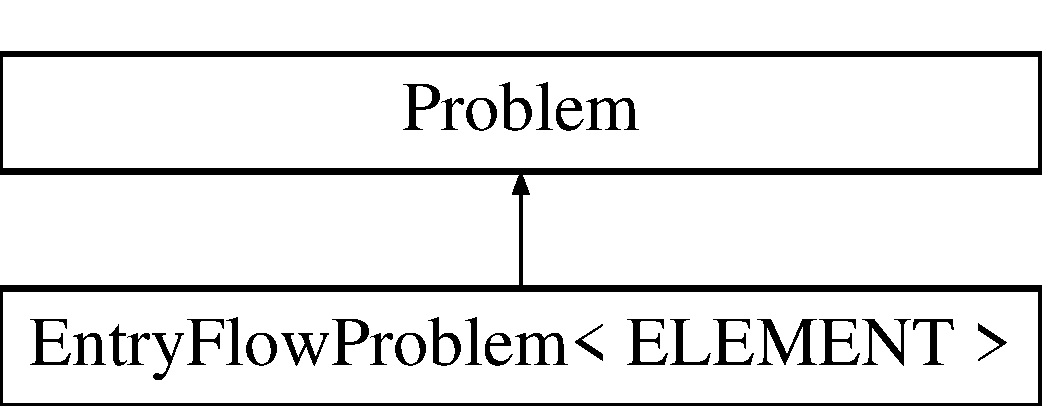
\includegraphics[height=2.000000cm]{classEntryFlowProblem}
\end{center}
\end{figure}
\subsection*{Public Member Functions}
\begin{DoxyCompactItemize}
\item 
\hyperlink{classEntryFlowProblem_a0d527811321d270d769224dcbac8d240}{Entry\+Flow\+Problem} (Doc\+Info \&doc\+\_\+info, const double \&min\+\_\+error\+\_\+target, const double \&max\+\_\+error\+\_\+target)
\begin{DoxyCompactList}\small\item\em Constructor\+: Pass Doc\+Info object and target errors. \end{DoxyCompactList}\item 
\hyperlink{classEntryFlowProblem_a22d76abde64459f167067c1d2cb5c1e2}{$\sim$\+Entry\+Flow\+Problem} ()
\begin{DoxyCompactList}\small\item\em Destructor (empty) \end{DoxyCompactList}\item 
void \hyperlink{classEntryFlowProblem_a034e6085f31de2c44419090b64d503db}{actions\+\_\+after\+\_\+newton\+\_\+solve} ()
\begin{DoxyCompactList}\small\item\em Doc the solution after solve. \end{DoxyCompactList}\item 
void \hyperlink{classEntryFlowProblem_ae4dde95573350d8fdb19463849991130}{actions\+\_\+before\+\_\+newton\+\_\+solve} ()
\begin{DoxyCompactList}\small\item\em Update the problem specs before solve. \end{DoxyCompactList}\item 
void \hyperlink{classEntryFlowProblem_ae472a4319c372d33ee22dac8fb32d9a2}{actions\+\_\+after\+\_\+adapt} ()
\begin{DoxyCompactList}\small\item\em After adaptation\+: Pin redudant pressure dofs. \end{DoxyCompactList}\item 
void \hyperlink{classEntryFlowProblem_a8ba37cd2a4af4356e4182929027d7828}{doc\+\_\+solution} ()
\begin{DoxyCompactList}\small\item\em Doc the solution. \end{DoxyCompactList}\item 
Refineable\+Quarter\+Tube\+Mesh$<$ E\+L\+E\+M\+E\+NT $>$ $\ast$ \hyperlink{classEntryFlowProblem_a4a880eeef280b621728ecceea42fe3ff}{mesh\+\_\+pt} ()
\begin{DoxyCompactList}\small\item\em Overload generic access function by one that returns a pointer to the specific mesh. \end{DoxyCompactList}\end{DoxyCompactItemize}
\subsection*{Private Attributes}
\begin{DoxyCompactItemize}
\item 
int \hyperlink{classEntryFlowProblem_a4b69957951a6367b12bf02c1a8d9ad2a}{Alpha}
\begin{DoxyCompactList}\small\item\em Exponent for bluntness of velocity profile. \end{DoxyCompactList}\item 
Doc\+Info \hyperlink{classEntryFlowProblem_abf50dd060db0e4c31628cfd228e096b8}{Doc\+\_\+info}
\begin{DoxyCompactList}\small\item\em Doc info object. \end{DoxyCompactList}\end{DoxyCompactItemize}


\subsection{Detailed Description}
\subsubsection*{template$<$class E\+L\+E\+M\+E\+NT$>$\newline
class Entry\+Flow\+Problem$<$ E\+L\+E\+M\+E\+N\+T $>$}

Entry flow problem in quarter tube domain. 

Definition at line 57 of file three\+\_\+d\+\_\+entry\+\_\+flow.\+cc.



\subsection{Constructor \& Destructor Documentation}
\mbox{\Hypertarget{classEntryFlowProblem_a0d527811321d270d769224dcbac8d240}\label{classEntryFlowProblem_a0d527811321d270d769224dcbac8d240}} 
\index{Entry\+Flow\+Problem@{Entry\+Flow\+Problem}!Entry\+Flow\+Problem@{Entry\+Flow\+Problem}}
\index{Entry\+Flow\+Problem@{Entry\+Flow\+Problem}!Entry\+Flow\+Problem@{Entry\+Flow\+Problem}}
\subsubsection{\texorpdfstring{Entry\+Flow\+Problem()}{EntryFlowProblem()}}
{\footnotesize\ttfamily template$<$class E\+L\+E\+M\+E\+NT $>$ \\
\hyperlink{classEntryFlowProblem}{Entry\+Flow\+Problem}$<$ E\+L\+E\+M\+E\+NT $>$\+::\hyperlink{classEntryFlowProblem}{Entry\+Flow\+Problem} (\begin{DoxyParamCaption}\item[{Doc\+Info \&}]{doc\+\_\+info,  }\item[{const double \&}]{min\+\_\+error\+\_\+target,  }\item[{const double \&}]{max\+\_\+error\+\_\+target }\end{DoxyParamCaption})}



Constructor\+: Pass Doc\+Info object and target errors. 

Constructor\+: Pass Doc\+Info object and error targets. 

Definition at line 117 of file three\+\_\+d\+\_\+entry\+\_\+flow.\+cc.



References Entry\+Flow\+Problem$<$ E\+L\+E\+M\+E\+N\+T $>$\+::\+Alpha, Entry\+Flow\+Problem$<$ E\+L\+E\+M\+E\+N\+T $>$\+::mesh\+\_\+pt(), and Global\+\_\+\+Physical\+\_\+\+Variables\+::\+Re.

\mbox{\Hypertarget{classEntryFlowProblem_a22d76abde64459f167067c1d2cb5c1e2}\label{classEntryFlowProblem_a22d76abde64459f167067c1d2cb5c1e2}} 
\index{Entry\+Flow\+Problem@{Entry\+Flow\+Problem}!````~Entry\+Flow\+Problem@{$\sim$\+Entry\+Flow\+Problem}}
\index{````~Entry\+Flow\+Problem@{$\sim$\+Entry\+Flow\+Problem}!Entry\+Flow\+Problem@{Entry\+Flow\+Problem}}
\subsubsection{\texorpdfstring{$\sim$\+Entry\+Flow\+Problem()}{~EntryFlowProblem()}}
{\footnotesize\ttfamily template$<$class E\+L\+E\+M\+E\+NT$>$ \\
\hyperlink{classEntryFlowProblem}{Entry\+Flow\+Problem}$<$ E\+L\+E\+M\+E\+NT $>$\+::$\sim$\hyperlink{classEntryFlowProblem}{Entry\+Flow\+Problem} (\begin{DoxyParamCaption}{ }\end{DoxyParamCaption})\hspace{0.3cm}{\ttfamily [inline]}}



Destructor (empty) 



Definition at line 67 of file three\+\_\+d\+\_\+entry\+\_\+flow.\+cc.



\subsection{Member Function Documentation}
\mbox{\Hypertarget{classEntryFlowProblem_ae472a4319c372d33ee22dac8fb32d9a2}\label{classEntryFlowProblem_ae472a4319c372d33ee22dac8fb32d9a2}} 
\index{Entry\+Flow\+Problem@{Entry\+Flow\+Problem}!actions\+\_\+after\+\_\+adapt@{actions\+\_\+after\+\_\+adapt}}
\index{actions\+\_\+after\+\_\+adapt@{actions\+\_\+after\+\_\+adapt}!Entry\+Flow\+Problem@{Entry\+Flow\+Problem}}
\subsubsection{\texorpdfstring{actions\+\_\+after\+\_\+adapt()}{actions\_after\_adapt()}}
{\footnotesize\ttfamily template$<$class E\+L\+E\+M\+E\+NT$>$ \\
void \hyperlink{classEntryFlowProblem}{Entry\+Flow\+Problem}$<$ E\+L\+E\+M\+E\+NT $>$\+::actions\+\_\+after\+\_\+adapt (\begin{DoxyParamCaption}{ }\end{DoxyParamCaption})\hspace{0.3cm}{\ttfamily [inline]}}



After adaptation\+: Pin redudant pressure dofs. 



Definition at line 83 of file three\+\_\+d\+\_\+entry\+\_\+flow.\+cc.

\mbox{\Hypertarget{classEntryFlowProblem_a034e6085f31de2c44419090b64d503db}\label{classEntryFlowProblem_a034e6085f31de2c44419090b64d503db}} 
\index{Entry\+Flow\+Problem@{Entry\+Flow\+Problem}!actions\+\_\+after\+\_\+newton\+\_\+solve@{actions\+\_\+after\+\_\+newton\+\_\+solve}}
\index{actions\+\_\+after\+\_\+newton\+\_\+solve@{actions\+\_\+after\+\_\+newton\+\_\+solve}!Entry\+Flow\+Problem@{Entry\+Flow\+Problem}}
\subsubsection{\texorpdfstring{actions\+\_\+after\+\_\+newton\+\_\+solve()}{actions\_after\_newton\_solve()}}
{\footnotesize\ttfamily template$<$class E\+L\+E\+M\+E\+NT$>$ \\
void \hyperlink{classEntryFlowProblem}{Entry\+Flow\+Problem}$<$ E\+L\+E\+M\+E\+NT $>$\+::actions\+\_\+after\+\_\+newton\+\_\+solve (\begin{DoxyParamCaption}{ }\end{DoxyParamCaption})\hspace{0.3cm}{\ttfamily [inline]}}



Doc the solution after solve. 



Definition at line 70 of file three\+\_\+d\+\_\+entry\+\_\+flow.\+cc.

\mbox{\Hypertarget{classEntryFlowProblem_ae4dde95573350d8fdb19463849991130}\label{classEntryFlowProblem_ae4dde95573350d8fdb19463849991130}} 
\index{Entry\+Flow\+Problem@{Entry\+Flow\+Problem}!actions\+\_\+before\+\_\+newton\+\_\+solve@{actions\+\_\+before\+\_\+newton\+\_\+solve}}
\index{actions\+\_\+before\+\_\+newton\+\_\+solve@{actions\+\_\+before\+\_\+newton\+\_\+solve}!Entry\+Flow\+Problem@{Entry\+Flow\+Problem}}
\subsubsection{\texorpdfstring{actions\+\_\+before\+\_\+newton\+\_\+solve()}{actions\_before\_newton\_solve()}}
{\footnotesize\ttfamily template$<$class E\+L\+E\+M\+E\+NT $>$ \\
void \hyperlink{classEntryFlowProblem}{Entry\+Flow\+Problem}$<$ E\+L\+E\+M\+E\+NT $>$\+::actions\+\_\+before\+\_\+newton\+\_\+solve (\begin{DoxyParamCaption}{ }\end{DoxyParamCaption})}



Update the problem specs before solve. 

Set the inflow boundary conditions. 

Definition at line 247 of file three\+\_\+d\+\_\+entry\+\_\+flow.\+cc.



References Entry\+Flow\+Problem$<$ E\+L\+E\+M\+E\+N\+T $>$\+::\+Alpha, and Entry\+Flow\+Problem$<$ E\+L\+E\+M\+E\+N\+T $>$\+::mesh\+\_\+pt().

\mbox{\Hypertarget{classEntryFlowProblem_a8ba37cd2a4af4356e4182929027d7828}\label{classEntryFlowProblem_a8ba37cd2a4af4356e4182929027d7828}} 
\index{Entry\+Flow\+Problem@{Entry\+Flow\+Problem}!doc\+\_\+solution@{doc\+\_\+solution}}
\index{doc\+\_\+solution@{doc\+\_\+solution}!Entry\+Flow\+Problem@{Entry\+Flow\+Problem}}
\subsubsection{\texorpdfstring{doc\+\_\+solution()}{doc\_solution()}}
{\footnotesize\ttfamily template$<$class E\+L\+E\+M\+E\+NT $>$ \\
void \hyperlink{classEntryFlowProblem}{Entry\+Flow\+Problem}$<$ E\+L\+E\+M\+E\+NT $>$\+::doc\+\_\+solution (\begin{DoxyParamCaption}{ }\end{DoxyParamCaption})}



Doc the solution. 



Definition at line 275 of file three\+\_\+d\+\_\+entry\+\_\+flow.\+cc.



References Entry\+Flow\+Problem$<$ E\+L\+E\+M\+E\+N\+T $>$\+::\+Doc\+\_\+info, and Entry\+Flow\+Problem$<$ E\+L\+E\+M\+E\+N\+T $>$\+::mesh\+\_\+pt().



Referenced by main().

\mbox{\Hypertarget{classEntryFlowProblem_a4a880eeef280b621728ecceea42fe3ff}\label{classEntryFlowProblem_a4a880eeef280b621728ecceea42fe3ff}} 
\index{Entry\+Flow\+Problem@{Entry\+Flow\+Problem}!mesh\+\_\+pt@{mesh\+\_\+pt}}
\index{mesh\+\_\+pt@{mesh\+\_\+pt}!Entry\+Flow\+Problem@{Entry\+Flow\+Problem}}
\subsubsection{\texorpdfstring{mesh\+\_\+pt()}{mesh\_pt()}}
{\footnotesize\ttfamily template$<$class E\+L\+E\+M\+E\+NT$>$ \\
Refineable\+Quarter\+Tube\+Mesh$<$E\+L\+E\+M\+E\+NT$>$$\ast$ \hyperlink{classEntryFlowProblem}{Entry\+Flow\+Problem}$<$ E\+L\+E\+M\+E\+NT $>$\+::mesh\+\_\+pt (\begin{DoxyParamCaption}{ }\end{DoxyParamCaption})\hspace{0.3cm}{\ttfamily [inline]}}



Overload generic access function by one that returns a pointer to the specific mesh. 



Definition at line 95 of file three\+\_\+d\+\_\+entry\+\_\+flow.\+cc.



Referenced by Entry\+Flow\+Problem$<$ E\+L\+E\+M\+E\+N\+T $>$\+::actions\+\_\+before\+\_\+newton\+\_\+solve(), Entry\+Flow\+Problem$<$ E\+L\+E\+M\+E\+N\+T $>$\+::doc\+\_\+solution(), and Entry\+Flow\+Problem$<$ E\+L\+E\+M\+E\+N\+T $>$\+::\+Entry\+Flow\+Problem().



\subsection{Member Data Documentation}
\mbox{\Hypertarget{classEntryFlowProblem_a4b69957951a6367b12bf02c1a8d9ad2a}\label{classEntryFlowProblem_a4b69957951a6367b12bf02c1a8d9ad2a}} 
\index{Entry\+Flow\+Problem@{Entry\+Flow\+Problem}!Alpha@{Alpha}}
\index{Alpha@{Alpha}!Entry\+Flow\+Problem@{Entry\+Flow\+Problem}}
\subsubsection{\texorpdfstring{Alpha}{Alpha}}
{\footnotesize\ttfamily template$<$class E\+L\+E\+M\+E\+NT$>$ \\
int \hyperlink{classEntryFlowProblem}{Entry\+Flow\+Problem}$<$ E\+L\+E\+M\+E\+NT $>$\+::Alpha\hspace{0.3cm}{\ttfamily [private]}}



Exponent for bluntness of velocity profile. 



Definition at line 103 of file three\+\_\+d\+\_\+entry\+\_\+flow.\+cc.



Referenced by Entry\+Flow\+Problem$<$ E\+L\+E\+M\+E\+N\+T $>$\+::actions\+\_\+before\+\_\+newton\+\_\+solve(), and Entry\+Flow\+Problem$<$ E\+L\+E\+M\+E\+N\+T $>$\+::\+Entry\+Flow\+Problem().

\mbox{\Hypertarget{classEntryFlowProblem_abf50dd060db0e4c31628cfd228e096b8}\label{classEntryFlowProblem_abf50dd060db0e4c31628cfd228e096b8}} 
\index{Entry\+Flow\+Problem@{Entry\+Flow\+Problem}!Doc\+\_\+info@{Doc\+\_\+info}}
\index{Doc\+\_\+info@{Doc\+\_\+info}!Entry\+Flow\+Problem@{Entry\+Flow\+Problem}}
\subsubsection{\texorpdfstring{Doc\+\_\+info}{Doc\_info}}
{\footnotesize\ttfamily template$<$class E\+L\+E\+M\+E\+NT$>$ \\
Doc\+Info \hyperlink{classEntryFlowProblem}{Entry\+Flow\+Problem}$<$ E\+L\+E\+M\+E\+NT $>$\+::Doc\+\_\+info\hspace{0.3cm}{\ttfamily [private]}}



Doc info object. 



Definition at line 106 of file three\+\_\+d\+\_\+entry\+\_\+flow.\+cc.



Referenced by Entry\+Flow\+Problem$<$ E\+L\+E\+M\+E\+N\+T $>$\+::doc\+\_\+solution().



The documentation for this class was generated from the following file\+:\begin{DoxyCompactItemize}
\item 
\hyperlink{three__d__entry__flow_8cc}{three\+\_\+d\+\_\+entry\+\_\+flow.\+cc}\end{DoxyCompactItemize}

\hypertarget{classMyCylinder}{}\section{My\+Cylinder Class Reference}
\label{classMyCylinder}\index{My\+Cylinder@{My\+Cylinder}}
Inheritance diagram for My\+Cylinder\+:\begin{figure}[H]
\begin{center}
\leavevmode
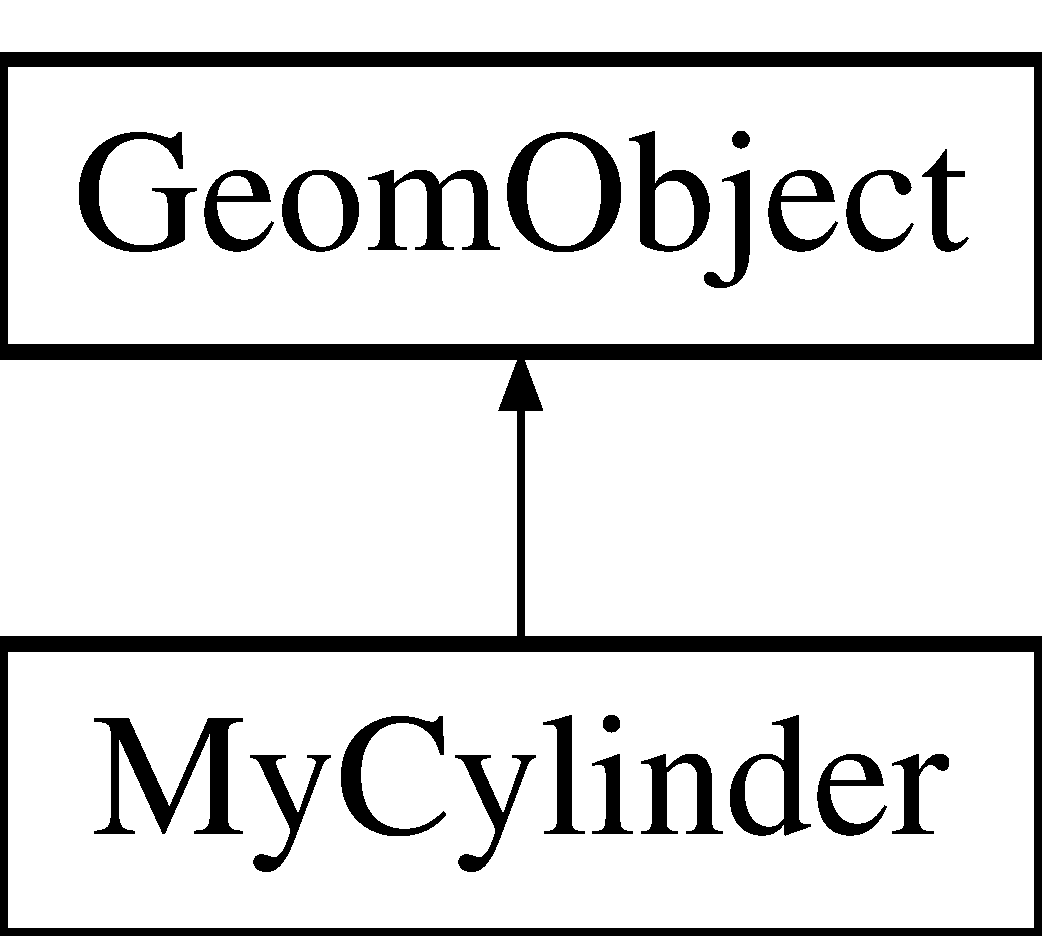
\includegraphics[height=2.000000cm]{classMyCylinder}
\end{center}
\end{figure}
\subsection*{Public Member Functions}
\begin{DoxyCompactItemize}
\item 
\hyperlink{classMyCylinder_ab4794e9b1b43d02e62cfe660b902e469}{My\+Cylinder} (const double \&radius)
\begin{DoxyCompactList}\small\item\em Constructor that takes the radius of the tube as its argument. \end{DoxyCompactList}\item 
virtual \hyperlink{classMyCylinder_ab886e268e53bd295cc2d220a96e93bd9}{$\sim$\+My\+Cylinder} ()
\begin{DoxyCompactList}\small\item\em Destructor. \end{DoxyCompactList}\item 
void \hyperlink{classMyCylinder_add84f8717aa286d627ae9175e0c27d4a}{position} (const Vector$<$ double $>$ \&xi, Vector$<$ double $>$ \&r) const
\begin{DoxyCompactList}\small\item\em Lagrangian coordinate xi. \end{DoxyCompactList}\item 
void \hyperlink{classMyCylinder_a6ba18b398d0626bd14d7cc8c5873b8a2}{position} (const unsigned \&t, const Vector$<$ double $>$ \&xi, Vector$<$ double $>$ \&r) const
\end{DoxyCompactItemize}
\subsection*{Private Attributes}
\begin{DoxyCompactItemize}
\item 
double \hyperlink{classMyCylinder_a3151803ae1fbe1a9858fca37b0f0f20b}{Radius}
\begin{DoxyCompactList}\small\item\em Storage for the radius of the tube. \end{DoxyCompactList}\end{DoxyCompactItemize}


\subsection{Detailed Description}


Definition at line 48 of file full\+\_\+tube.\+cc.



\subsection{Constructor \& Destructor Documentation}
\mbox{\Hypertarget{classMyCylinder_ab4794e9b1b43d02e62cfe660b902e469}\label{classMyCylinder_ab4794e9b1b43d02e62cfe660b902e469}} 
\index{My\+Cylinder@{My\+Cylinder}!My\+Cylinder@{My\+Cylinder}}
\index{My\+Cylinder@{My\+Cylinder}!My\+Cylinder@{My\+Cylinder}}
\subsubsection{\texorpdfstring{My\+Cylinder()}{MyCylinder()}}
{\footnotesize\ttfamily My\+Cylinder\+::\+My\+Cylinder (\begin{DoxyParamCaption}\item[{const double \&}]{radius }\end{DoxyParamCaption})\hspace{0.3cm}{\ttfamily [inline]}}



Constructor that takes the radius of the tube as its argument. 



Definition at line 53 of file full\+\_\+tube.\+cc.

\mbox{\Hypertarget{classMyCylinder_ab886e268e53bd295cc2d220a96e93bd9}\label{classMyCylinder_ab886e268e53bd295cc2d220a96e93bd9}} 
\index{My\+Cylinder@{My\+Cylinder}!````~My\+Cylinder@{$\sim$\+My\+Cylinder}}
\index{````~My\+Cylinder@{$\sim$\+My\+Cylinder}!My\+Cylinder@{My\+Cylinder}}
\subsubsection{\texorpdfstring{$\sim$\+My\+Cylinder()}{~MyCylinder()}}
{\footnotesize\ttfamily virtual My\+Cylinder\+::$\sim$\+My\+Cylinder (\begin{DoxyParamCaption}{ }\end{DoxyParamCaption})\hspace{0.3cm}{\ttfamily [inline]}}



Destructor. 



Definition at line 57 of file full\+\_\+tube.\+cc.



\subsection{Member Function Documentation}
\mbox{\Hypertarget{classMyCylinder_add84f8717aa286d627ae9175e0c27d4a}\label{classMyCylinder_add84f8717aa286d627ae9175e0c27d4a}} 
\index{My\+Cylinder@{My\+Cylinder}!position@{position}}
\index{position@{position}!My\+Cylinder@{My\+Cylinder}}
\subsubsection{\texorpdfstring{position()}{position()}\hspace{0.1cm}{\footnotesize\ttfamily [1/2]}}
{\footnotesize\ttfamily void My\+Cylinder\+::position (\begin{DoxyParamCaption}\item[{const Vector$<$ double $>$ \&}]{xi,  }\item[{Vector$<$ double $>$ \&}]{r }\end{DoxyParamCaption}) const\hspace{0.3cm}{\ttfamily [inline]}}



Lagrangian coordinate xi. 



Definition at line 60 of file full\+\_\+tube.\+cc.

\mbox{\Hypertarget{classMyCylinder_a6ba18b398d0626bd14d7cc8c5873b8a2}\label{classMyCylinder_a6ba18b398d0626bd14d7cc8c5873b8a2}} 
\index{My\+Cylinder@{My\+Cylinder}!position@{position}}
\index{position@{position}!My\+Cylinder@{My\+Cylinder}}
\subsubsection{\texorpdfstring{position()}{position()}\hspace{0.1cm}{\footnotesize\ttfamily [2/2]}}
{\footnotesize\ttfamily void My\+Cylinder\+::position (\begin{DoxyParamCaption}\item[{const unsigned \&}]{t,  }\item[{const Vector$<$ double $>$ \&}]{xi,  }\item[{Vector$<$ double $>$ \&}]{r }\end{DoxyParamCaption}) const\hspace{0.3cm}{\ttfamily [inline]}}

Return the position of the tube as a function of time (doesn\textquotesingle{}t move as a function of time) 

Definition at line 70 of file full\+\_\+tube.\+cc.



\subsection{Member Data Documentation}
\mbox{\Hypertarget{classMyCylinder_a3151803ae1fbe1a9858fca37b0f0f20b}\label{classMyCylinder_a3151803ae1fbe1a9858fca37b0f0f20b}} 
\index{My\+Cylinder@{My\+Cylinder}!Radius@{Radius}}
\index{Radius@{Radius}!My\+Cylinder@{My\+Cylinder}}
\subsubsection{\texorpdfstring{Radius}{Radius}}
{\footnotesize\ttfamily double My\+Cylinder\+::\+Radius\hspace{0.3cm}{\ttfamily [private]}}



Storage for the radius of the tube. 



Definition at line 79 of file full\+\_\+tube.\+cc.



The documentation for this class was generated from the following file\+:\begin{DoxyCompactItemize}
\item 
\hyperlink{full__tube_8cc}{full\+\_\+tube.\+cc}\end{DoxyCompactItemize}

\hypertarget{classSteadyTubeProblem}{}\section{Steady\+Tube\+Problem$<$ E\+L\+E\+M\+E\+NT $>$ Class Template Reference}
\label{classSteadyTubeProblem}\index{Steady\+Tube\+Problem$<$ E\+L\+E\+M\+E\+N\+T $>$@{Steady\+Tube\+Problem$<$ E\+L\+E\+M\+E\+N\+T $>$}}


Entry flow problem in tapered tube domain.  


Inheritance diagram for Steady\+Tube\+Problem$<$ E\+L\+E\+M\+E\+NT $>$\+:\begin{figure}[H]
\begin{center}
\leavevmode
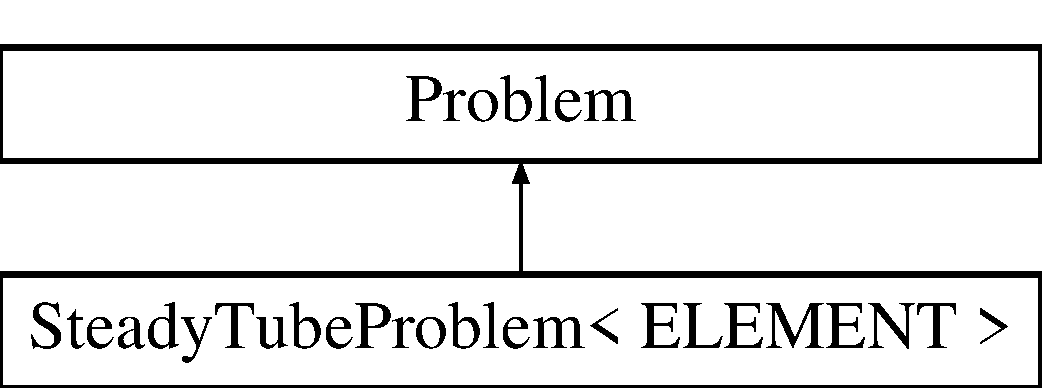
\includegraphics[height=2.000000cm]{classSteadyTubeProblem}
\end{center}
\end{figure}
\subsection*{Public Member Functions}
\begin{DoxyCompactItemize}
\item 
\hyperlink{classSteadyTubeProblem_a333c59fbeb36a2a5cbb170fc34783ec4}{Steady\+Tube\+Problem} (Doc\+Info \&doc\+\_\+info, const double \&min\+\_\+error\+\_\+target, const double \&max\+\_\+error\+\_\+target)
\begin{DoxyCompactList}\small\item\em Constructor\+: Pass Doc\+Info object and target errors. \end{DoxyCompactList}\item 
\hyperlink{classSteadyTubeProblem_a1564d3faf03e6724565097e730d099d5}{$\sim$\+Steady\+Tube\+Problem} ()
\begin{DoxyCompactList}\small\item\em Destructor (empty) \end{DoxyCompactList}\item 
void \hyperlink{classSteadyTubeProblem_a5c5277cac2a887dc6c85892e9f851f97}{actions\+\_\+before\+\_\+newton\+\_\+solve} ()
\begin{DoxyCompactList}\small\item\em Update the problem specs before solve. \end{DoxyCompactList}\item 
void \hyperlink{classSteadyTubeProblem_ae598a2a0ec9bbfb563a1c78aa159561f}{actions\+\_\+after\+\_\+adapt} ()
\begin{DoxyCompactList}\small\item\em After adaptation\+: Pin redudant pressure dofs. \end{DoxyCompactList}\item 
void \hyperlink{classSteadyTubeProblem_ae384d816cf88c86e9f18549701d791f8}{doc\+\_\+solution} ()
\begin{DoxyCompactList}\small\item\em Doc the solution. \end{DoxyCompactList}\item 
Refineable\+Tube\+Mesh$<$ E\+L\+E\+M\+E\+NT $>$ $\ast$ \hyperlink{classSteadyTubeProblem_ac2f2254773b6e20c58a104f9a12efba8}{mesh\+\_\+pt} ()
\begin{DoxyCompactList}\small\item\em Overload generic access function by one that returns a pointer to the specific mesh. \end{DoxyCompactList}\end{DoxyCompactItemize}
\subsection*{Private Attributes}
\begin{DoxyCompactItemize}
\item 
Doc\+Info \hyperlink{classSteadyTubeProblem_a2d535b7b21eb6383b9f3c9f4c3ce4510}{Doc\+\_\+info}
\begin{DoxyCompactList}\small\item\em Doc info object. \end{DoxyCompactList}\item 
Geom\+Object $\ast$ \hyperlink{classSteadyTubeProblem_aedad3a2d2afd1f1c306dae289b3c2baf}{Volume\+\_\+pt}
\begin{DoxyCompactList}\small\item\em Pointer to Geom\+Object that specifies the domain volume. \end{DoxyCompactList}\end{DoxyCompactItemize}


\subsection{Detailed Description}
\subsubsection*{template$<$class E\+L\+E\+M\+E\+NT$>$\newline
class Steady\+Tube\+Problem$<$ E\+L\+E\+M\+E\+N\+T $>$}

Entry flow problem in tapered tube domain. 

Definition at line 98 of file full\+\_\+tube.\+cc.



\subsection{Constructor \& Destructor Documentation}
\mbox{\Hypertarget{classSteadyTubeProblem_a333c59fbeb36a2a5cbb170fc34783ec4}\label{classSteadyTubeProblem_a333c59fbeb36a2a5cbb170fc34783ec4}} 
\index{Steady\+Tube\+Problem@{Steady\+Tube\+Problem}!Steady\+Tube\+Problem@{Steady\+Tube\+Problem}}
\index{Steady\+Tube\+Problem@{Steady\+Tube\+Problem}!Steady\+Tube\+Problem@{Steady\+Tube\+Problem}}
\subsubsection{\texorpdfstring{Steady\+Tube\+Problem()}{SteadyTubeProblem()}}
{\footnotesize\ttfamily template$<$class E\+L\+E\+M\+E\+NT $>$ \\
\hyperlink{classSteadyTubeProblem}{Steady\+Tube\+Problem}$<$ E\+L\+E\+M\+E\+NT $>$\+::\hyperlink{classSteadyTubeProblem}{Steady\+Tube\+Problem} (\begin{DoxyParamCaption}\item[{Doc\+Info \&}]{doc\+\_\+info,  }\item[{const double \&}]{min\+\_\+error\+\_\+target,  }\item[{const double \&}]{max\+\_\+error\+\_\+target }\end{DoxyParamCaption})}



Constructor\+: Pass Doc\+Info object and target errors. 

Constructor\+: Pass Doc\+Info object and error targets. 

Definition at line 148 of file full\+\_\+tube.\+cc.



References Steady\+Tube\+Problem$<$ E\+L\+E\+M\+E\+N\+T $>$\+::mesh\+\_\+pt(), Global\+\_\+\+Physical\+\_\+\+Variables\+::\+Re, and Steady\+Tube\+Problem$<$ E\+L\+E\+M\+E\+N\+T $>$\+::\+Volume\+\_\+pt.

\mbox{\Hypertarget{classSteadyTubeProblem_a1564d3faf03e6724565097e730d099d5}\label{classSteadyTubeProblem_a1564d3faf03e6724565097e730d099d5}} 
\index{Steady\+Tube\+Problem@{Steady\+Tube\+Problem}!````~Steady\+Tube\+Problem@{$\sim$\+Steady\+Tube\+Problem}}
\index{````~Steady\+Tube\+Problem@{$\sim$\+Steady\+Tube\+Problem}!Steady\+Tube\+Problem@{Steady\+Tube\+Problem}}
\subsubsection{\texorpdfstring{$\sim$\+Steady\+Tube\+Problem()}{~SteadyTubeProblem()}}
{\footnotesize\ttfamily template$<$class E\+L\+E\+M\+E\+NT$>$ \\
\hyperlink{classSteadyTubeProblem}{Steady\+Tube\+Problem}$<$ E\+L\+E\+M\+E\+NT $>$\+::$\sim$\hyperlink{classSteadyTubeProblem}{Steady\+Tube\+Problem} (\begin{DoxyParamCaption}{ }\end{DoxyParamCaption})\hspace{0.3cm}{\ttfamily [inline]}}



Destructor (empty) 



Definition at line 108 of file full\+\_\+tube.\+cc.



\subsection{Member Function Documentation}
\mbox{\Hypertarget{classSteadyTubeProblem_ae598a2a0ec9bbfb563a1c78aa159561f}\label{classSteadyTubeProblem_ae598a2a0ec9bbfb563a1c78aa159561f}} 
\index{Steady\+Tube\+Problem@{Steady\+Tube\+Problem}!actions\+\_\+after\+\_\+adapt@{actions\+\_\+after\+\_\+adapt}}
\index{actions\+\_\+after\+\_\+adapt@{actions\+\_\+after\+\_\+adapt}!Steady\+Tube\+Problem@{Steady\+Tube\+Problem}}
\subsubsection{\texorpdfstring{actions\+\_\+after\+\_\+adapt()}{actions\_after\_adapt()}}
{\footnotesize\ttfamily template$<$class E\+L\+E\+M\+E\+NT$>$ \\
void \hyperlink{classSteadyTubeProblem}{Steady\+Tube\+Problem}$<$ E\+L\+E\+M\+E\+NT $>$\+::actions\+\_\+after\+\_\+adapt (\begin{DoxyParamCaption}{ }\end{DoxyParamCaption})\hspace{0.3cm}{\ttfamily [inline]}}



After adaptation\+: Pin redudant pressure dofs. 



Definition at line 114 of file full\+\_\+tube.\+cc.

\mbox{\Hypertarget{classSteadyTubeProblem_a5c5277cac2a887dc6c85892e9f851f97}\label{classSteadyTubeProblem_a5c5277cac2a887dc6c85892e9f851f97}} 
\index{Steady\+Tube\+Problem@{Steady\+Tube\+Problem}!actions\+\_\+before\+\_\+newton\+\_\+solve@{actions\+\_\+before\+\_\+newton\+\_\+solve}}
\index{actions\+\_\+before\+\_\+newton\+\_\+solve@{actions\+\_\+before\+\_\+newton\+\_\+solve}!Steady\+Tube\+Problem@{Steady\+Tube\+Problem}}
\subsubsection{\texorpdfstring{actions\+\_\+before\+\_\+newton\+\_\+solve()}{actions\_before\_newton\_solve()}}
{\footnotesize\ttfamily template$<$class E\+L\+E\+M\+E\+NT $>$ \\
void \hyperlink{classSteadyTubeProblem}{Steady\+Tube\+Problem}$<$ E\+L\+E\+M\+E\+NT $>$\+::actions\+\_\+before\+\_\+newton\+\_\+solve (\begin{DoxyParamCaption}{ }\end{DoxyParamCaption})}



Update the problem specs before solve. 

Set the inflow boundary conditions. 

Definition at line 255 of file full\+\_\+tube.\+cc.



References Steady\+Tube\+Problem$<$ E\+L\+E\+M\+E\+N\+T $>$\+::mesh\+\_\+pt().

\mbox{\Hypertarget{classSteadyTubeProblem_ae384d816cf88c86e9f18549701d791f8}\label{classSteadyTubeProblem_ae384d816cf88c86e9f18549701d791f8}} 
\index{Steady\+Tube\+Problem@{Steady\+Tube\+Problem}!doc\+\_\+solution@{doc\+\_\+solution}}
\index{doc\+\_\+solution@{doc\+\_\+solution}!Steady\+Tube\+Problem@{Steady\+Tube\+Problem}}
\subsubsection{\texorpdfstring{doc\+\_\+solution()}{doc\_solution()}}
{\footnotesize\ttfamily template$<$class E\+L\+E\+M\+E\+NT $>$ \\
void \hyperlink{classSteadyTubeProblem}{Steady\+Tube\+Problem}$<$ E\+L\+E\+M\+E\+NT $>$\+::doc\+\_\+solution (\begin{DoxyParamCaption}{ }\end{DoxyParamCaption})}



Doc the solution. 



Definition at line 282 of file full\+\_\+tube.\+cc.



References Steady\+Tube\+Problem$<$ E\+L\+E\+M\+E\+N\+T $>$\+::\+Doc\+\_\+info, Steady\+Tube\+Problem$<$ E\+L\+E\+M\+E\+N\+T $>$\+::mesh\+\_\+pt(), and Global\+\_\+\+Physical\+\_\+\+Variables\+::\+Re.



Referenced by main().

\mbox{\Hypertarget{classSteadyTubeProblem_ac2f2254773b6e20c58a104f9a12efba8}\label{classSteadyTubeProblem_ac2f2254773b6e20c58a104f9a12efba8}} 
\index{Steady\+Tube\+Problem@{Steady\+Tube\+Problem}!mesh\+\_\+pt@{mesh\+\_\+pt}}
\index{mesh\+\_\+pt@{mesh\+\_\+pt}!Steady\+Tube\+Problem@{Steady\+Tube\+Problem}}
\subsubsection{\texorpdfstring{mesh\+\_\+pt()}{mesh\_pt()}}
{\footnotesize\ttfamily template$<$class E\+L\+E\+M\+E\+NT$>$ \\
Refineable\+Tube\+Mesh$<$E\+L\+E\+M\+E\+NT$>$$\ast$ \hyperlink{classSteadyTubeProblem}{Steady\+Tube\+Problem}$<$ E\+L\+E\+M\+E\+NT $>$\+::mesh\+\_\+pt (\begin{DoxyParamCaption}{ }\end{DoxyParamCaption})\hspace{0.3cm}{\ttfamily [inline]}}



Overload generic access function by one that returns a pointer to the specific mesh. 



Definition at line 126 of file full\+\_\+tube.\+cc.



Referenced by Steady\+Tube\+Problem$<$ E\+L\+E\+M\+E\+N\+T $>$\+::actions\+\_\+before\+\_\+newton\+\_\+solve(), Steady\+Tube\+Problem$<$ E\+L\+E\+M\+E\+N\+T $>$\+::doc\+\_\+solution(), and Steady\+Tube\+Problem$<$ E\+L\+E\+M\+E\+N\+T $>$\+::\+Steady\+Tube\+Problem().



\subsection{Member Data Documentation}
\mbox{\Hypertarget{classSteadyTubeProblem_a2d535b7b21eb6383b9f3c9f4c3ce4510}\label{classSteadyTubeProblem_a2d535b7b21eb6383b9f3c9f4c3ce4510}} 
\index{Steady\+Tube\+Problem@{Steady\+Tube\+Problem}!Doc\+\_\+info@{Doc\+\_\+info}}
\index{Doc\+\_\+info@{Doc\+\_\+info}!Steady\+Tube\+Problem@{Steady\+Tube\+Problem}}
\subsubsection{\texorpdfstring{Doc\+\_\+info}{Doc\_info}}
{\footnotesize\ttfamily template$<$class E\+L\+E\+M\+E\+NT$>$ \\
Doc\+Info \hyperlink{classSteadyTubeProblem}{Steady\+Tube\+Problem}$<$ E\+L\+E\+M\+E\+NT $>$\+::Doc\+\_\+info\hspace{0.3cm}{\ttfamily [private]}}



Doc info object. 



Definition at line 134 of file full\+\_\+tube.\+cc.



Referenced by Steady\+Tube\+Problem$<$ E\+L\+E\+M\+E\+N\+T $>$\+::doc\+\_\+solution().

\mbox{\Hypertarget{classSteadyTubeProblem_aedad3a2d2afd1f1c306dae289b3c2baf}\label{classSteadyTubeProblem_aedad3a2d2afd1f1c306dae289b3c2baf}} 
\index{Steady\+Tube\+Problem@{Steady\+Tube\+Problem}!Volume\+\_\+pt@{Volume\+\_\+pt}}
\index{Volume\+\_\+pt@{Volume\+\_\+pt}!Steady\+Tube\+Problem@{Steady\+Tube\+Problem}}
\subsubsection{\texorpdfstring{Volume\+\_\+pt}{Volume\_pt}}
{\footnotesize\ttfamily template$<$class E\+L\+E\+M\+E\+NT$>$ \\
Geom\+Object$\ast$ \hyperlink{classSteadyTubeProblem}{Steady\+Tube\+Problem}$<$ E\+L\+E\+M\+E\+NT $>$\+::Volume\+\_\+pt\hspace{0.3cm}{\ttfamily [private]}}



Pointer to Geom\+Object that specifies the domain volume. 



Definition at line 137 of file full\+\_\+tube.\+cc.



Referenced by Steady\+Tube\+Problem$<$ E\+L\+E\+M\+E\+N\+T $>$\+::\+Steady\+Tube\+Problem().



The documentation for this class was generated from the following file\+:\begin{DoxyCompactItemize}
\item 
\hyperlink{full__tube_8cc}{full\+\_\+tube.\+cc}\end{DoxyCompactItemize}

\chapter{File Documentation}
\hypertarget{full__tube_8cc}{}\section{full\+\_\+tube.\+cc File Reference}
\label{full__tube_8cc}\index{full\+\_\+tube.\+cc@{full\+\_\+tube.\+cc}}
\subsection*{Classes}
\begin{DoxyCompactItemize}
\item 
class \hyperlink{classMyCylinder}{My\+Cylinder}
\item 
class \hyperlink{classSteadyTubeProblem}{Steady\+Tube\+Problem$<$ E\+L\+E\+M\+E\+N\+T $>$}
\begin{DoxyCompactList}\small\item\em Entry flow problem in tapered tube domain. \end{DoxyCompactList}\end{DoxyCompactItemize}
\subsection*{Namespaces}
\begin{DoxyCompactItemize}
\item 
 \hyperlink{namespaceGlobal__Physical__Variables}{Global\+\_\+\+Physical\+\_\+\+Variables}
\begin{DoxyCompactList}\small\item\em Namespace for physical parameters. \end{DoxyCompactList}\end{DoxyCompactItemize}
\subsection*{Functions}
\begin{DoxyCompactItemize}
\item 
int \hyperlink{full__tube_8cc_a0ddf1224851353fc92bfbff6f499fa97}{main} (int argc, char $\ast$argv\mbox{[}$\,$\mbox{]})
\begin{DoxyCompactList}\small\item\em Driver for 3D entry flow into a straight tube. \end{DoxyCompactList}\end{DoxyCompactItemize}
\subsection*{Variables}
\begin{DoxyCompactItemize}
\item 
double \hyperlink{namespaceGlobal__Physical__Variables_ab814e627d2eb5bc50318879d19ab16b9}{Global\+\_\+\+Physical\+\_\+\+Variables\+::\+Re} =25
\begin{DoxyCompactList}\small\item\em Reynolds number. \end{DoxyCompactList}\end{DoxyCompactItemize}


\subsection{Function Documentation}
\mbox{\Hypertarget{full__tube_8cc_a0ddf1224851353fc92bfbff6f499fa97}\label{full__tube_8cc_a0ddf1224851353fc92bfbff6f499fa97}} 
\index{full\+\_\+tube.\+cc@{full\+\_\+tube.\+cc}!main@{main}}
\index{main@{main}!full\+\_\+tube.\+cc@{full\+\_\+tube.\+cc}}
\subsubsection{\texorpdfstring{main()}{main()}}
{\footnotesize\ttfamily int main (\begin{DoxyParamCaption}\item[{int}]{argc,  }\item[{char $\ast$}]{argv\mbox{[}$\,$\mbox{]} }\end{DoxyParamCaption})}



Driver for 3D entry flow into a straight tube. 



Definition at line 314 of file full\+\_\+tube.\+cc.



References Steady\+Tube\+Problem$<$ E\+L\+E\+M\+E\+N\+T $>$\+::doc\+\_\+solution(), and Global\+\_\+\+Physical\+\_\+\+Variables\+::\+Re.


\hypertarget{three__d__entry__flow_8cc}{}\section{three\+\_\+d\+\_\+entry\+\_\+flow.\+cc File Reference}
\label{three__d__entry__flow_8cc}\index{three\+\_\+d\+\_\+entry\+\_\+flow.\+cc@{three\+\_\+d\+\_\+entry\+\_\+flow.\+cc}}
\subsection*{Classes}
\begin{DoxyCompactItemize}
\item 
class \hyperlink{classEntryFlowProblem}{Entry\+Flow\+Problem$<$ E\+L\+E\+M\+E\+N\+T $>$}
\begin{DoxyCompactList}\small\item\em Entry flow problem in quarter tube domain. \end{DoxyCompactList}\end{DoxyCompactItemize}
\subsection*{Namespaces}
\begin{DoxyCompactItemize}
\item 
 \hyperlink{namespaceGlobal__Physical__Variables}{Global\+\_\+\+Physical\+\_\+\+Variables}
\begin{DoxyCompactList}\small\item\em Namespace for physical parameters. \end{DoxyCompactList}\end{DoxyCompactItemize}
\subsection*{Functions}
\begin{DoxyCompactItemize}
\item 
int \hyperlink{three__d__entry__flow_8cc_a0ddf1224851353fc92bfbff6f499fa97}{main} (int argc, char $\ast$argv\mbox{[}$\,$\mbox{]})
\end{DoxyCompactItemize}


\subsection{Function Documentation}
\mbox{\Hypertarget{three__d__entry__flow_8cc_a0ddf1224851353fc92bfbff6f499fa97}\label{three__d__entry__flow_8cc_a0ddf1224851353fc92bfbff6f499fa97}} 
\index{three\+\_\+d\+\_\+entry\+\_\+flow.\+cc@{three\+\_\+d\+\_\+entry\+\_\+flow.\+cc}!main@{main}}
\index{main@{main}!three\+\_\+d\+\_\+entry\+\_\+flow.\+cc@{three\+\_\+d\+\_\+entry\+\_\+flow.\+cc}}
\subsubsection{\texorpdfstring{main()}{main()}}
{\footnotesize\ttfamily int main (\begin{DoxyParamCaption}\item[{int}]{argc,  }\item[{char $\ast$}]{argv\mbox{[}$\,$\mbox{]} }\end{DoxyParamCaption})}

Driver for 3D entry flow into a quarter tube. If there are any command line arguments, we regard this as a validation run and perform only a single adaptation 

Definition at line 307 of file three\+\_\+d\+\_\+entry\+\_\+flow.\+cc.



References Entry\+Flow\+Problem$<$ E\+L\+E\+M\+E\+N\+T $>$\+::doc\+\_\+solution().


\hypertarget{three__d__entry__flow_8txt__doxygenified_8h}{}\section{three\+\_\+d\+\_\+entry\+\_\+flow.\+txt\+\_\+doxygenified.\+h File Reference}
\label{three__d__entry__flow_8txt__doxygenified_8h}\index{three\+\_\+d\+\_\+entry\+\_\+flow.\+txt\+\_\+doxygenified.\+h@{three\+\_\+d\+\_\+entry\+\_\+flow.\+txt\+\_\+doxygenified.\+h}}

%--- End generated contents ---

% Index
\backmatter
\newpage
\phantomsection
\clearemptydoublepage
\addcontentsline{toc}{chapter}{Index}
\printindex

